\documentclass[t]{beamer}

% --- Theme and Color Setup ---
\usetheme{Madrid}

% Define the custom Orange color
\definecolor{MyOrange}{RGB}{230, 85, 10}

% Apply the orange color to the structure
\usecolortheme[named=MyOrange]{structure}

% Fix footer colors to match the orange theme
\setbeamercolor{palette primary}{bg=MyOrange,fg=white}
\setbeamercolor{palette secondary}{bg=MyOrange!80!black,fg=white}
\setbeamercolor{palette tertiary}{bg=MyOrange!60!black,fg=white}
\setbeamerfont{caption}{size=\footnotesize}

% Packages
\usepackage[utf8]{inputenc}
\usepackage{hyperref}
\usepackage{tikz}
\usepackage{booktabs}
\usepackage{amsmath}
\usepackage{graphicx}

% --- 1. CONFIGURATION FOR CONTENT SLIDES (Middle Pages) ---
\addtobeamertemplate{frametitle}{}{%
    \begin{tikzpicture}[remember picture,overlay]
        \node[anchor=north east, xshift=-0.3cm, yshift=0cm, inner sep=0pt] at (current page.north east) {
            \includegraphics[height=1cm, keepaspectratio]{logo_white.png}
        };
    \end{tikzpicture}%
}

% --- 2. CONFIGURATION FOR FIRST & LAST PAGE ---
\newcommand{\FirstLastPageLayout}{
    \begin{tikzpicture}[remember picture,overlay]
        \node[anchor=north east, xshift=-0.3cm, yshift=0cm, inner sep=0pt] at (current page.north east) {
            \includegraphics[height=1cm, keepaspectratio]{logo.jpg}
        };
        \node[anchor=south west, xshift=0.5cm, yshift=0.5cm] at (current page.south west) {
            \textcolor{MyOrange}{\footnotesize Prague University of Economics and Business}
        };
    \end{tikzpicture}
}

% --- Info ---
\title[HammingMesh + Jellyfish]{HammingMesh with Jellyfish Local Topology}
\subtitle{Thesis Progress Update}
\author{Kirk}
\institute[]{Department of International Economic Relations}
\date{\today}

\begin{document}

% --- Title Page ---
\begin{frame}
    \FirstLastPageLayout
    \titlepage
\end{frame}

% --- Contents ---
\begin{frame}{Contents}
    \begin{itemize}
        \item HammingMesh Overview
        \item Switch Types \& Port Assignments
        \item Routing
        \item Jellyfish Variant
        \item Diameter \& Bisection Bandwidth
        \item Benchmarks \& Results
    \end{itemize}
\end{frame}

% ===========================================================
% HAMMINGMESH OVERVIEW
% ===========================================================
\begin{frame}{HammingMesh -- Conceptual Overview}
    \begin{itemize}
        \item Two-level hierarchical topology for deep learning clusters

        \vspace{0.2cm}

        \item \textbf{Local level}: 2D mesh on each PCB board (cheap copper traces)
        \item \textbf{Global level}: Fat tree switches connecting boards row-wise and column-wise (fiber cables)

        \vspace{0.2cm}

        \item Key insight: DL communication is \textbf{toroidal} (rings along data/pipeline/operator axes) $\Rightarrow$ full bisection bandwidth not needed

        \vspace{0.2cm}

        \item \textbf{Naming}: Hx$a$Mesh = board with $a \times a$ switches
        \begin{itemize}
            \item Hx2Mesh: $2\times2$ boards (4 accelerators each)
            \item Hx4Mesh: $4\times4$ boards (16 accelerators each)
        \end{itemize}
    \end{itemize}
\end{frame}

% ===========================================================
% COORDINATE SYSTEM
% ===========================================================
\begin{frame}{Coordinate System}
    Every board switch is identified by a 4-tuple:
    \vspace{0.2cm}

    \centering
    \texttt{[a, b, x, y]}

    \vspace{0.2cm}

    \raggedright
    \begin{tabular}{cl}
        \toprule
        \textbf{Coord} & \textbf{Meaning} \\
        \midrule
        $a$ & Local row within the board \\
        $b$ & Local column within the board \\
        $x$ & Global row (which row of boards) \\
        $y$ & Global column (which column of boards) \\
        \bottomrule
    \end{tabular}

    \vspace{0.3cm}

    \textbf{Example}: Hx2Mesh, $2\times2$ global $\Rightarrow$ $2 \cdot 2 \cdot 2 \cdot 2 = 16$ nodes

    \textbf{Example}: Hx4Mesh, $8\times8$ global $\Rightarrow$ $4 \cdot 4 \cdot 8 \cdot 8 = 1024$ nodes
\end{frame}

% ===========================================================
% SWITCH TYPES & PORTS
% ===========================================================
\begin{frame}{Switch Types \& Port Assignments}
    \textbf{Board switches} -- 5 ports each:

    \vspace{0.2cm}

    \begin{tabular}{ccl}
        \toprule
        \textbf{Port} & \textbf{ID} & \textbf{Connects to} \\
        \midrule
        N & 0 & Mesh neighbor north \textit{or} column fat tree \\
        E & 1 & Mesh neighbor east \textit{or} row fat tree \\
        S & 2 & Mesh neighbor south \textit{or} column fat tree \\
        W & 3 & Mesh neighbor west \textit{or} row fat tree \\
        C & 4 & NIC (1 accelerator per switch) \\
        \bottomrule
    \end{tabular}

    \vspace{0.3cm}

    \textbf{Edge switches} serve dual purpose:
    \begin{itemize}
        \item Outward-facing port connects to \textbf{fat tree} instead of mesh neighbor
        \item West/East edges $\to$ row fat tree;~~North/South edges $\to$ column fat tree
    \end{itemize}
\end{frame}

% ===========================================================
% BOARD LAYOUT VISUAL
% ===========================================================
\begin{frame}{Board Layout (Hx4 Example)}
    \begin{center}
    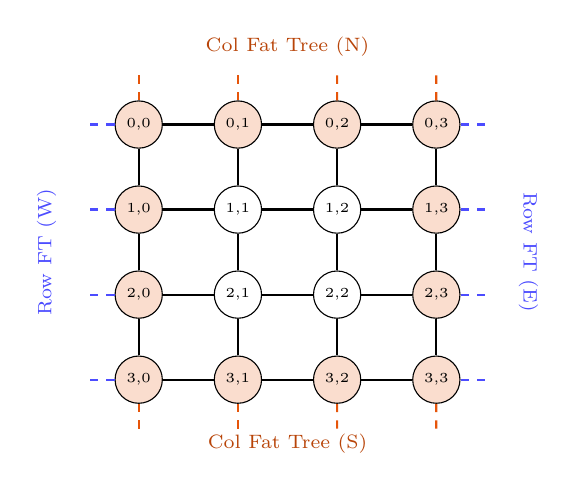
\begin{tikzpicture}[scale=0.9,
        switch/.style={circle, draw, fill=white, minimum size=6mm, inner sep=0pt, font=\tiny},
        edgeswitch/.style={circle, draw, fill=MyOrange!20, minimum size=6mm, inner sep=0pt, font=\tiny},
        ftlabel/.style={font=\scriptsize, text=MyOrange!80!black}
    ]
        % Draw 4x4 grid of switches
        \foreach \r in {0,...,3} {
            \foreach \c in {0,...,3} {
                \pgfmathtruncatemacro{\isedge}{(\r==0)||(\r==3)||(\c==0)||(\c==3) ? 1 : 0}
                \ifnum\isedge=1
                    \node[edgeswitch] (s\r\c) at (\c*1.4, -\r*1.2) {\r,\c};
                \else
                    \node[switch] (s\r\c) at (\c*1.4, -\r*1.2) {\r,\c};
                \fi
            }
        }
        % Horizontal mesh links
        \foreach \r in {0,...,3} {
            \foreach \c in {0,...,2} {
                \pgfmathtruncatemacro{\cnext}{\c+1}
                \draw[thick] (s\r\c) -- (s\r\cnext);
            }
        }
        % Vertical mesh links
        \foreach \r in {0,...,2} {
            \foreach \c in {0,...,3} {
                \pgfmathtruncatemacro{\rnext}{\r+1}
                \draw[thick] (s\r\c) -- (s\rnext\c);
            }
        }
        % Column fat tree (North)
        \foreach \c in {0,...,3} {
            \draw[MyOrange, thick, dashed] (s0\c) -- ++(0, 0.8);
        }
        \node[ftlabel] at (2.1, 1.1) {Col Fat Tree (N)};
        % Column fat tree (South)
        \foreach \c in {0,...,3} {
            \draw[MyOrange, thick, dashed] (s3\c) -- ++(0, -0.8);
        }
        \node[ftlabel] at (2.1, -4.5) {Col Fat Tree (S)};
        % Row fat tree (West)
        \foreach \r in {0,...,3} {
            \draw[blue!70, thick, dashed] (s\r0) -- ++(-0.8, 0);
        }
        \node[ftlabel, text=blue!70, rotate=90] at (-1.3, -1.8) {Row FT (W)};
        % Row fat tree (East)
        \foreach \r in {0,...,3} {
            \draw[blue!70, thick, dashed] (s\r3) -- ++(0.8, 0);
        }
        \node[ftlabel, text=blue!70, rotate=-90] at (5.5, -1.8) {Row FT (E)};
    \end{tikzpicture}
    \end{center}

    \vspace{-0.1cm}
    \footnotesize
    \colorbox{MyOrange!20}{\strut Edge switches}: outward port to fat tree. White: all 4 ports to mesh neighbors.
\end{frame}

% ===========================================================
% FAT TREE SWITCHES
% ===========================================================
\begin{frame}{Fat Tree Switches}
    Fat tree switches have \textbf{no NIC ports} -- all ports are router-to-router.

    \vspace{0.3cm}

    \textbf{Single-switch} (when boards fit one switch):
    \begin{itemize}
        \item All ports are down-ports to board edge switches
    \end{itemize}

    \vspace{0.2cm}

    \textbf{Two-level fat tree} (larger topologies):

    \vspace{0.1cm}
    \begin{tabular}{lll}
        \toprule
        \textbf{Level} & \textbf{Down ports} & \textbf{Up ports} \\
        \midrule
        0 (Edge) & To board edges & To core switches \\
        1 (Core) & To edge switches & -- \\
        \bottomrule
    \end{tabular}

    \vspace{0.3cm}

    \textbf{Two independent sets}:
    \begin{itemize}
        \item Row fat trees: handle East--West global connectivity
        \item Column fat trees: handle North--South global connectivity
    \end{itemize}
\end{frame}

% ===========================================================
% ROUTING
% ===========================================================
\begin{frame}{Routing -- Mesh HammingMesh}
    \textbf{4 routing cases} based on source/destination boards:

    \vspace{0.2cm}

    \begin{enumerate}
        \item \textbf{Same board}: route within local mesh (N/S/E/W). May wrap through fat tree if shorter.

        \item \textbf{Different row, same column}: head to nearest N/S edge $\to$ column fat tree

        \item \textbf{Same row, different column}: head to nearest E/W edge $\to$ row fat tree

        \item \textbf{Different row and column}: head to nearest board edge in any direction
    \end{enumerate}

    \vspace{0.2cm}

    \textbf{Adaptive}: among valid candidate ports, pick the one with most available output buffer credits (congestion-aware).

    \vspace{0.2cm}

    \textbf{Deadlock avoidance}: North-last routing + virtual channel escalation at board$\to$fat tree boundary.
\end{frame}

% ===========================================================
% JELLYFISH VARIANT
% ===========================================================
\begin{frame}{Jellyfish Variant -- Motivation}
    \begin{itemize}
        \item Replace the structured 2D mesh \textbf{within each board} with a \textbf{random regular graph} (Jellyfish)
        \item Global fat tree interconnect remains \textbf{unchanged}

        \vspace{0.3cm}

        \item \textbf{Why?} Random graphs can provide:
        \begin{itemize}
            \item Shorter average path lengths
            \item Higher bisection bandwidth
            \item More flexible incremental expansion
        \end{itemize}
        \ldots for the same node degree

        \vspace{0.3cm}

        \item Goal: evaluate if random local connectivity improves performance while keeping the HxMesh global hierarchy
    \end{itemize}
\end{frame}

\begin{frame}{Jellyfish -- Port Budget \& Graph Generation}
    \textbf{Port budget}: same 5 ports per switch, edge ports still reserved for fat trees.

    \vspace{0.1cm}
    \footnotesize
    \begin{tabular}{lccc}
        \toprule
        \textbf{Node type} & \textbf{Jellyfish links} & \textbf{Fat tree ports} & \textbf{NIC} \\
        \midrule
        Interior  & 4 & 0 & 1 \\
        Row-edge  & 3 & 1 & 1 \\
        Col-edge  & 3 & 1 & 1 \\
        Corner    & 2 & 2 & 1 \\
        \bottomrule
    \end{tabular}
    \normalsize

    \vspace{0.3cm}

    \textbf{Graph generation} (per board):
    \begin{enumerate}
        \item Collect free (non-reserved) ports as ``stubs''
        \item Shuffle stubs randomly
        \item Greedily pair stubs from different nodes (no self-loops, no duplicate links)
        \item If unpaired stubs remain $\to$ retry with new shuffle (up to 100 attempts)
    \end{enumerate}
\end{frame}

\begin{frame}{Jellyfish -- Board Layout (4\texttimes4 Board, 16 nodes)}
    \begin{columns}[c]
        \begin{column}{0.48\textwidth}
            \centering
            \textbf{Mesh (structured)}
            \vspace{0.15cm}

            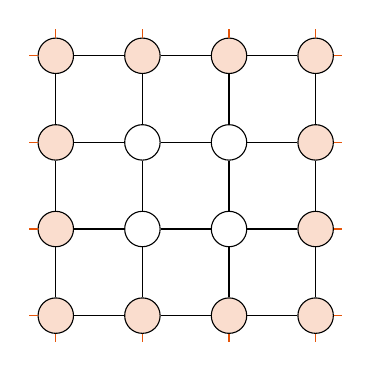
\begin{tikzpicture}[
                sw/.style={circle,draw,fill=white,minimum size=4.5mm,inner sep=0pt},
                esw/.style={circle,draw,fill=MyOrange!20,minimum size=4.5mm,inner sep=0pt},
                ftlink/.style={MyOrange,thin,dashed},
                ml/.style={black,thin}
            ]
                % Nodes: edge=orange, interior=white
                \foreach \r in {0,...,3} {
                    \foreach \c in {0,...,3} {
                        \pgfmathtruncatemacro{\isedge}{(\r==0)||\r==3||(\c==0)||\c==3 ? 1 : 0}
                        \ifnum\isedge=1
                            \node[esw] (m\r\c) at (\c*1.1,-\r*1.1) {};
                        \else
                            \node[sw]  (m\r\c) at (\c*1.1,-\r*1.1) {};
                        \fi
                    }
                }
                % Horizontal mesh links
                \foreach \r in {0,...,3} {
                    \foreach \c in {0,...,2} {
                        \pgfmathtruncatemacro{\nc}{\c+1}
                        \draw[ml] (m\r\c)--(m\r\nc);
                    }
                }
                % Vertical mesh links
                \foreach \r in {0,...,2} {
                    \foreach \c in {0,...,3} {
                        \pgfmathtruncatemacro{\nr}{\r+1}
                        \draw[ml] (m\r\c)--(m\nr\c);
                    }
                }
                % Fat tree stubs
                \foreach \c in {0,...,3} { \draw[ftlink] (m0\c)--++(0,0.35); }
                \foreach \c in {0,...,3} { \draw[ftlink] (m3\c)--++(0,-0.35); }
                \foreach \r in {0,...,3} { \draw[ftlink] (m\r0)--++(-0.35,0); }
                \foreach \r in {0,...,3} { \draw[ftlink] (m\r3)--++(0.35,0); }
            \end{tikzpicture}
        \end{column}
        \begin{column}{0.04\textwidth}
            \centering\large$\Rightarrow$
        \end{column}
        \begin{column}{0.48\textwidth}
            \centering
            \textbf{Jellyfish (random)}
            \vspace{0.15cm}

            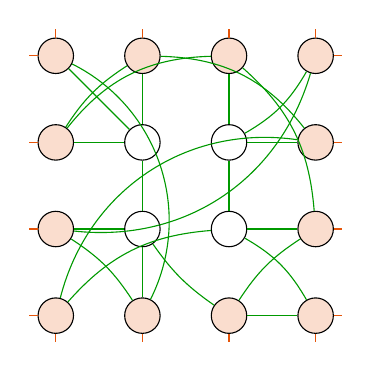
\begin{tikzpicture}[
                sw/.style={circle,draw,fill=white,minimum size=4.5mm,inner sep=0pt},
                esw/.style={circle,draw,fill=MyOrange!20,minimum size=4.5mm,inner sep=0pt},
                ftlink/.style={MyOrange,thin,dashed},
                jl/.style={green!60!black,thin}
            ]
                % Nodes: edge=orange, interior=white
                \foreach \r in {0,...,3} {
                    \foreach \c in {0,...,3} {
                        \pgfmathtruncatemacro{\isedge}{(\r==0)||(\r==3)||(\c==0)||(\c==3) ? 1 : 0}
                        \ifnum\isedge=1
                            \node[esw] (j\r\c) at (\c*1.1,-\r*1.1) {};
                        \else
                            \node[sw]  (j\r\c) at (\c*1.1,-\r*1.1) {};
                        \fi
                    }
                }
                % --- Valid random Jellyfish graph (24 links, degrees: corners=2, edges=3, interior=4) ---
                % Short / adjacent links
                \draw[jl] (j00)--(j11);
                \draw[jl] (j01)--(j11);
                \draw[jl] (j10)--(j11);
                \draw[jl] (j11)--(j21);
                \draw[jl] (j02)--(j12);
                \draw[jl] (j03) to[bend left=15] (j12);
                \draw[jl] (j12)--(j13);
                \draw[jl] (j12)--(j22);
                \draw[jl] (j20)--(j21);
                \draw[jl] (j21)--(j31);
                \draw[jl] (j21) to[bend right=10] (j32);
                \draw[jl] (j22)--(j23);
                \draw[jl] (j32)--(j33);
                \draw[jl] (j01) to[bend right=12] (j10);
                \draw[jl] (j20) to[bend left=12] (j31);
                \draw[jl] (j23) to[bend right=12] (j32);
                % Medium-range links
                \draw[jl] (j01) to[bend left=25] (j13);
                \draw[jl] (j02) to[bend right=25] (j10);
                \draw[jl] (j02) to[bend left=22] (j23);
                \draw[jl] (j22) to[bend right=22] (j30);
                \draw[jl] (j22) to[bend left=15] (j33);
                % Long-range links (arc outside to stay readable)
                \draw[jl] (j00) to[bend left=45] (j31);
                \draw[jl] (j03) to[bend left=40] (j20);
                \draw[jl] (j13) to[bend right=42] (j30);
                % Fat tree stubs
                \foreach \c in {0,...,3} { \draw[ftlink] (j0\c)--++(0,0.35); }
                \foreach \c in {0,...,3} { \draw[ftlink] (j3\c)--++(0,-0.35); }
                \foreach \r in {0,...,3} { \draw[ftlink] (j\r0)--++(-0.35,0); }
                \foreach \r in {0,...,3} { \draw[ftlink] (j\r3)--++(0.35,0); }
            \end{tikzpicture}
        \end{column}
    \end{columns}

    \vspace{0.15cm}
    \footnotesize
    \colorbox{MyOrange!20}{\strut~Edge nodes~} reserve ports for fat trees.
    \textcolor{green!60!black}{\textbf{Green}}: random Jellyfish links (24 total).
    \textcolor{MyOrange}{\textbf{Dashed}}: fat tree (unchanged).
\end{frame}

\begin{frame}{Jellyfish -- Routing}
    Mesh directional routing does not work for random graphs.

    \vspace{0.2cm}

    $\Rightarrow$ \textbf{Table-based shortest-path routing}:

    \begin{enumerate}
        \item BFS computes routing tables in Python for each board
        \item Tables passed to C++ as comma-separated parameters
        \item \texttt{routing\_table[dest\_local\_id]} = next hop port
    \end{enumerate}

    \vspace{0.2cm}

    \textbf{Three cases} in \texttt{route\_packet\_jellyfish()}:
    \begin{itemize}
        \item \textbf{Same switch}: deliver to NIC
        \item \textbf{Same board}: follow \texttt{routing\_table[dest]}
        \item \textbf{Different board}: route to nearest edge node (row or column, depending on which fat tree is needed), then exit to fat tree
    \end{itemize}

    \vspace{0.2cm}

    Each node stores \texttt{nearest\_row\_edge} and \texttt{nearest\_col\_edge} for fast edge lookup.
\end{frame}

% ===========================================================
% DIAMETER
% ===========================================================
\begin{frame}{Diameter Comparison}
    \textbf{Mesh-based HammingMesh} (fat tree global):
    \[D_{\text{mesh}} =
    3\left\lfloor \frac{a-1}{2} \right\rfloor
    + 4\left\lceil \frac{1}{3}\log_{\lceil x^{1/3}\rceil}\!\left(x\right) \right\rceil
    + 4\left\lceil \frac{1}{3}\log_{\lceil y^{1/3}\rceil}\!\left(y\right) \right\rceil
    \]

    \vspace{0.2cm}

    \textbf{Jellyfish-based HammingMesh} (Jellyfish diameter $\approx 3$):
    \[D_{\text{jelly}} =
    9
    + 4\left\lceil \frac{1}{3}\log_{\lceil x^{1/3}\rceil}\!\left(x\right) \right\rceil
    + 4\left\lceil \frac{1}{3}\log_{\lceil y^{1/3}\rceil}\!\left(y\right) \right\rceil
    \]

    \vspace{0.2cm}

    For flat topology (single switch): $D_{\text{mesh,flat}} = 2(\lfloor\frac{a-1}{2}\rfloor + 1)$ vs.\ $D_{\text{jelly,flat}} = 8$

    \vspace{0.2cm}

    \footnotesize
    Jellyfish replaces $3\lfloor\frac{a-1}{2}\rfloor$ with a constant 9 -- advantageous for larger boards ($a \geq 4$).
\end{frame}

% ===========================================================
% BISECTION BANDWIDTH
% ===========================================================
\begin{frame}{Bisection Bandwidth}
    Bisection cut occurs \textbf{between boards}, not within them.

    \vspace{0.2cm}

    For Hx$a$Mesh with $x \times y$ boards (cutting along $y$):
    \[B_{\text{bisection}} = 2ax \cdot BW\]

    \vspace{0.2cm}

    \textbf{Same formula for both mesh and Jellyfish variants} -- the bisection depends on global connections, not local topology.

    \vspace{0.3cm}

    \textbf{Scalability}: Jellyfish local topology supports incremental expansion via link rewiring, without rebuilding the fat tree.
\end{frame}

% ===========================================================
% BENCHMARKS
% ===========================================================
\begin{frame}{Benchmarks -- Setup}
    \textbf{Simulation}: SST 11.1.0 (cycle-accurate packet-level)

    \vspace{0.2cm}

    \textbf{Configuration}: Hx2Mesh, $2\times2$ boards, $2\times2$ global = \textbf{16 nodes}

    \vspace{0.2cm}

    \textbf{Topologies compared}: Hx2Mesh (mesh) vs.\ Hx2Mesh (Jellyfish)

    \vspace{0.3cm}

    \textbf{Benchmarks run}:
    \begin{enumerate}
        \item \textbf{AllToAll} -- every node sends to every other node (global bandwidth)
        \item \textbf{AllReduce} -- ring-based reduction (ring0.5D variant)
        \item \textbf{Random Permutation} -- each node sends 2$\times$32\,MiB to a random partner (per-node bandwidth distribution)
    \end{enumerate}

    \vspace{0.2cm}

    \footnotesize
    Paper also includes: ResNet-152, CosmoFlow, GPT-3, GPT-3 MoE, DLRM
\end{frame}

% ===========================================================
% RESULTS -- AllToAll
% ===========================================================
\begin{frame}{Results -- AllToAll (16 nodes)}
    \begin{figure}
        \centering
        \includegraphics[width=0.85\textwidth]{all_to_all.png}
    \end{figure}

    \vspace{-0.3cm}
    \begin{itemize}
        \item Both topologies converge to $\sim$500 Gb/s at large message sizes
        \item Jellyfish slightly higher at mid-range sizes (2--8\,KB)
        \item At 16 nodes, local topology differences have limited impact on global all-to-all traffic
    \end{itemize}
\end{frame}

% ===========================================================
% RESULTS -- AllReduce
% ===========================================================
\begin{frame}{Results -- AllReduce (16 nodes)}
    \begin{figure}
        \centering
        \includegraphics[width=0.75\textwidth]{all_reduce.png}
    \end{figure}

    \vspace{-0.3cm}
    \begin{itemize}
        \item Mesh: $\sim$460 Gb/s (near torus theoretical max)
        \item Jellyfish: $\sim$180 Gb/s -- significantly lower
        \item Ring AllReduce relies on structured neighbor ordering; random graph disrupts optimal ring mapping
    \end{itemize}
\end{frame}

% ===========================================================
% RESULTS -- Random Permutation
% ===========================================================
\begin{frame}{Results -- Random Permutation (16 nodes)}
    \begin{figure}
        \centering
        \includegraphics[width=0.75\textwidth]{random_perm.png}
    \end{figure}

    \vspace{-0.3cm}
    \begin{itemize}
        \item Mesh: median $\sim$420 Gb/s, tighter distribution
        \item Jellyfish: median $\sim$300 Gb/s, wider variance
        \item Random graph creates uneven path lengths $\to$ more variance in per-node bandwidth
    \end{itemize}
\end{frame}

% ===========================================================
% SUMMARY & NEXT STEPS
% ===========================================================
\begin{frame}{Summary \& Next Steps}
    \textbf{Observations so far} (16-node topology):
    \begin{itemize}
        \item AllToAll: comparable performance (both $\sim$500 Gb/s)
        \item AllReduce: mesh significantly outperforms Jellyfish (460 vs 180 Gb/s)
        \item Random Permutation: mesh has higher median and less variance
    \end{itemize}

    \vspace{0.3cm}

    \textbf{Next steps}:
    \begin{itemize}
        \item Run benchmarks at larger scale (256, 1024 nodes)
        \item Run DNN workloads: ResNet, CosmoFlow, GPT-3, DLRM
        \item Investigate Jellyfish AllReduce regression (ring mapping on random graphs)
        \item Compare with other topologies from the paper (fat tree, Dragonfly, torus)
    \end{itemize}
\end{frame}

% --- Final page ---
\begin{frame}[c]
    \FirstLastPageLayout
    \centering
    \Huge \textcolor{MyOrange}{Thank you}

    \vspace{1.5cm}
    \normalsize
    \textbf{Kirk}
\end{frame}

\end{document}
